% 无封面页
\documentclass[withoutpreface]{cumcmthesis}

\begin{document}
    %% 摘要页
    \begin{abstractpage}{基于优劣解距离法(TOPSIS)的河流评价系统}
            
        本文主要解决如何建立合理的数学评价体系,来对具有多重指标的河流水质进行量化评价。

        针对所要研究的问题,我们采用了\textbf{优劣解距离法( TOPSIS )}行建模。首先,我们分别确定了各指标的类型,并将非极大型指标转化为极大型指标,即进行了\textbf{指标正向化}。然后,我们通过\textbf{标准化}消除了量纲的影响,并定义了最优解和最劣解,计算出各个评价对象与最优解、最劣解之间的距离。最后,我们根据这些距离,得出了最终的河流打分并进行了可视化排序。

        我们还指出了改进模型的方法:通过层次分析法和熵权法等其他方法引入指标权重,以得到更加精确、更加科学的得分结论。

        \keywords{评价 \quad 距离 \quad TOPSIS \quad 指标正向化 \quad 标准化}

    \end{abstractpage}

    %% 目录页
    \tocpage

    \section{问题重述}

    已知有河流 A-T ,其水质数据如\cref{Tab:1}所示。请建立合理的数学评价模型,对这些河流的水质进行打分和排序。

    \begin{table}[H]
        \centering
        \caption{河流水质数据}\label{Tab:1}
        \begin{tabular}{|c|c|c|c|c|}
        \hline
        \textbf{河流} & \multicolumn{1}{c|}{\textbf{含氧量( ppm )}} & \multicolumn{1}{c|}{\textbf{PH 值}} & \multicolumn{1}{c|}{\textbf{细菌总数(个/mL)}} & \multicolumn{1}{c|}{\textcolor[rgb]{ .2,  .2,  .2}{\textbf{植物性营养物量( ppm )}}} \bigstrut\\
        \hline
        A     & 4.69  & 6.59  & 51    & 11.94 \bigstrut\\
        \hline
        B     & 2.03  & 7.86  & 19    & 6.46 \bigstrut\\
        \hline
        C     & 9.11  & 6.31  & 46    & 8.91 \bigstrut\\
        \hline
        D     & 8.61  & 7.05  & 46    & 26.43 \bigstrut\\
        \hline
        E     & 7.13  & 6.5   & 50    & 23.57 \bigstrut\\
        \hline
        F     & 2.39  & 6.77  & 38    & 24.62 \bigstrut\\
        \hline
        G     & 7.69  & 6.79  & 38    & 6.01 \bigstrut\\
        \hline
        H     & 9.3   & 6.81  & 27    & 31.57 \bigstrut\\
        \hline
        I     & 5.45  & 7.62  & 5     & 18.46 \bigstrut\\
        \hline
        J     & 6.19  & 7.27  & 17    & 7.51 \bigstrut\\
        \hline
        K     & 7.93  & 7.53  & 9     & 6.52 \bigstrut\\
        \hline
        L     & 4.4   & 7.28  & 17    & 25.3 \bigstrut\\
        \hline
        M     & 7.46  & 8.24  & 23    & 14.42 \bigstrut\\
        \hline
        N     & 2.01  & 5.55  & 47    & 26.31 \bigstrut\\
        \hline
        O     & 2.04  & 6.4   & 23    & 17.91 \bigstrut\\
        \hline
        P     & 7.73  & 6.14  & 52    & 15.72 \bigstrut\\
        \hline
        Q     & 6.35  & 7.58  & 25    & 29.46 \bigstrut\\
        \hline
        R     & 8.29  & 8.41  & 39    & 12.02 \bigstrut\\
        \hline
        S     & 3.54  & 7.27  & 54    & 3.16 \bigstrut\\
        \hline
        T     & 7.44  & 6.26  & 8     & 28.41 \bigstrut\\
        \hline
        \end{tabular}
    \end{table}

    \section{问题分析}

    本题是一道含数据的多指标评价类问题。题中给出了衡量水质的4个指标以及各条河流的指标数据。我们可以采用TOPSIS方法: 构造最优方案和最劣方案,通过计算每个方案与最优方案和最劣方案之间的距离来衡量方案的优劣,并得出打分,进行排序。

    \section{模型假设}

    为了确保模型的有效性及方便后续建模,我们作出以下合理假设:

    \begin{itemize}
        \item 河流水质完全由数据中所给的4个指标决定
    \end{itemize}

    \section{符号假设}

    在此对本文使用到的一些符号作以下说明(未作说明则在文中详述):

    \begin{table}[H]
        \centering
        \caption{符号假设}\label{Tab:2}
        \begin{tabular}{p{30pt}<{\centering}|p{100pt}<{\centering}@{}p{260pt}<{\centering}}
        \hline
        \rowcolor{color2} 序号 & 符号 & 符号说明 \\
        \hline
        \rowcolor{color1} 1 & $\mathbf{X},\mathbf{Z}$		& 指标矩阵 \\
        \rowcolor{color1} 2 & m & 评价对象个数 \\
        \rowcolor{color1} 3 & n & 指标数\\
        \rowcolor{color1} 4 & $\omega$		& 权重向量 \\
        \rowcolor{color1} 4 & $(*)^+$		& 最优解相关的量 \\
        \rowcolor{color1} 4 & $(*)^-$		& 最劣解相关的量 \\
        \hline
        \end{tabular}
    \end{table}

    \section{模型简介}

    C.L. Hwang 和 K. Yoon 于1981年首次提出 TOPSIS (Technique for Order Preference by Similarity to an Ideal Solution),可译为逼近理想解排序法,国内常简称为优劣解距离法。

    TOPSIS 法是一种常用的综合评价方法,能充分利用原始数据的
    信息,其结果能精确地反映各评价方案之间的差距。

    基本过程为先将原始数据矩阵统一指标类型(一般正向化处理)
    得到正向化的矩阵,再对正向化的矩阵进行标准化处理以消除各指
    标量纲的影响,并找到有限方案中的最优方案和最劣方案,然后分
    别计算各评价对象与最优方案和最劣方案间的距离,获得各评价对
    象与最优方案的相对接近程度,以此作为评价优劣的依据。该方法
    对数据分布及样本含量没有严格限制,数据计算简单易行。

    \section{模型建立}

    \subsection{指标正向化}

    经过查阅资料,我们得到关于4个指标的相关信息,如\cref{Tab:3}所示。

    \begin{table}[H]
        \centering
        \caption{指标类型}\label{Tab:3}
        \begin{tabular}{ccc}
            \toprule[1.5pt]
            \makebox[0.2\textwidth][c]{指标} & \makebox[0.3\textwidth][c]{类型} & \makebox[0.4\textwidth][c]{含义} \\
            \midrule
            含氧量	&  极大型 & 越高越好 \\
            PH 值  & 中间型(7) & 越接近7越好 \\
            细菌总数 & 极小型 & 越少越好 \\ 
            植物性营养物量 & 区间型$([10-20])$ &  介于10-20之间最佳\\
            \bottomrule[1.5pt]
        \end{tabular}
    \end{table}

    为了使用 TOPSIS ,我们需要将非极大型指标转化为极大型指标,即进行所谓\textbf{指标正向化}。

    \subsubsection{极小型指标正向化}

    极小型指标正向化的方法比较简单。
    
    假设需要进行指标正向化的指标向量为$$\mathbf{x}=\begin{bmatrix}
        x_1  \\ x_2 \\ \vdots \\ x_m
    \end{bmatrix}$$
    
    则根据\cref{Eq:1},就可以计算得到指标正向化后的指标向量
    $$\mathbf{x}'=\begin{bmatrix}
        x_1'  \\ x_2' \\ \vdots \\ x_m'
    \end{bmatrix}$$
    \begin{equation}\label{Eq:1}
        x_i' = \max\mathbf{x}-x_i
    \end{equation}

    \subsubsection{中间型值指标正向化}
    
    假设需要进行指标正向化的指标向量为$$\mathbf{x}=\begin{bmatrix}
        x_1 \\ x_2 \\ \vdots \\ x_m
    \end{bmatrix}$$ 
    
    中间值为$x_0$,则根据\cref{Eq:2},就可以计算得到指标正向化后的指标向量
    $$\mathbf{x}'=\begin{bmatrix}
        x_1' \\ x_2' \\ \vdots \\ x_m'
    \end{bmatrix}$$
    \begin{equation*}
        M=\max (|\mathbf{x}-x_0|)
    \end{equation*}
    \begin{equation}\label{Eq:2}
        x_i' = 1 - \frac{|x_i-x_0|}{M}
    \end{equation}

    \subsubsection{区间型值指标正向化}
    
    假设需要进行指标正向化的指标向量为$$\mathbf{x}=\begin{bmatrix}
        x_1 \\ x_2 \\ \vdots \\ x_m
    \end{bmatrix}$$
    
    最佳区间为$[a,b]$,则根据\cref{Eq:3},就可以计算得到指标正向化后的指标向量
    $$\mathbf{x}'=\begin{bmatrix}
        x_1' \\ x_2' \\ \vdots \\ x_m'
    \end{bmatrix}$$
    \begin{equation*}
        M=\max \{a-\min \mathbf{x},\max \mathbf{x}-b\}
    \end{equation*}
    \begin{equation}\label{Eq:3}
        x_i'=\begin{cases}
            1-\frac{a-x_i}{M} & x_i<a \\ 
            1 & a\le x_i \le b \\ 
            1-\frac{x_i-b}{M} & x_i>b \\
        \end{cases}
    \end{equation}

    \subsection{正向化矩阵标准化}

    指标正向化个后,各个指标的量纲依然不同。为了消除不同量纲的影响,可以将正向化矩阵进行标准化。标准化的方法有很多。这里我们选择较为常见的一种。

    假设正向化矩阵为
    $$\mathbf{X}=\begin{bmatrix}
        x_{11} & x_{12} & \cdots & x_{1n} \\ 
        x_{21} & x_{22} & \cdots & x_{2n} \\
        \vdots & \vdots & \ddots & \vdots \\ 
        x_{m1} & x_{m2} & \cdots & x_{mn} \\
    \end{bmatrix}$$

    那么标准化后的矩阵$Z$的每个元素
    \begin{equation}
        z_{ij} = \frac{x_{ij}}{\sqrt{\sum\limits_{i=1}^{m}} x_{ij}^2}
    \end{equation}

    \subsection{计算得分并归一化}

    假设标准化后的矩阵
    $$\mathbf{Z}=\begin{bmatrix}
        z_{11} & z_{12} & \cdots & z_{1n} \\ 
        z_{21} & z_{22} & \cdots & z_{2n} \\
        \vdots & \vdots & \ddots & \vdots \\ 
        z_{m1} & z_{m2} & \cdots & z_{mn} \\
    \end{bmatrix}$$

    定义最优解$$Z^+ 
    =\begin{bmatrix} Z_1^+ & Z_2^+ & \cdots & Z_n^+\end{bmatrix}=
    $$
    $$
    \begin{bmatrix} \max\{z_{11},z_{12},\cdots,z_{1n}\} & \max\{z_{21},z_{22},\cdots,z_{2n}\} & \cdots & \max\{z_{n1},z_{n2},\cdots,z_{mn}\}\end{bmatrix}$$

    定义最劣解$$Z^- 
    =\begin{bmatrix} Z_1^- & Z_2^- & \cdots & Z_n^-\end{bmatrix}=
    $$
    $$
    \begin{bmatrix} \min\{z_{11},z_{12},\cdots,z_{1n}\} & \min\{z_{21},z_{22},\cdots,z_{2n}\} & \cdots & \min\{z_{n1},z_{n2},\cdots,z_{mn}\}\end{bmatrix}$$

    定义第 $i(i=1,2,\cdots,m)$ 个评价对象到最优解的距离 $D_i^+=\sqrt{\sum\limits_{j=1}^{n}(Z_j^+-z_{ij})^2}$

    定义第 $i(i=1,2,\cdots,m)$ 个评价对象到最劣解的距离 $D_i^-=\sqrt{\sum\limits_{j=1}^{n}(Z_j^--z_{ij})^2}$

    则我们可以以指标$\displaystyle S_i=\frac{D_i^+}{D_i^++D_i^-}$来衡量任意一个评价对象的优劣程度

    将$S_i$按照$$S_i'=\frac{S_i}{\sum\limits_{i=1}^{m}S_i}$$归一化后,即可得到最后的得分。

    最后的得分如\cref{Fig:1}所示

    \begin{figure}[H]
        \centering
        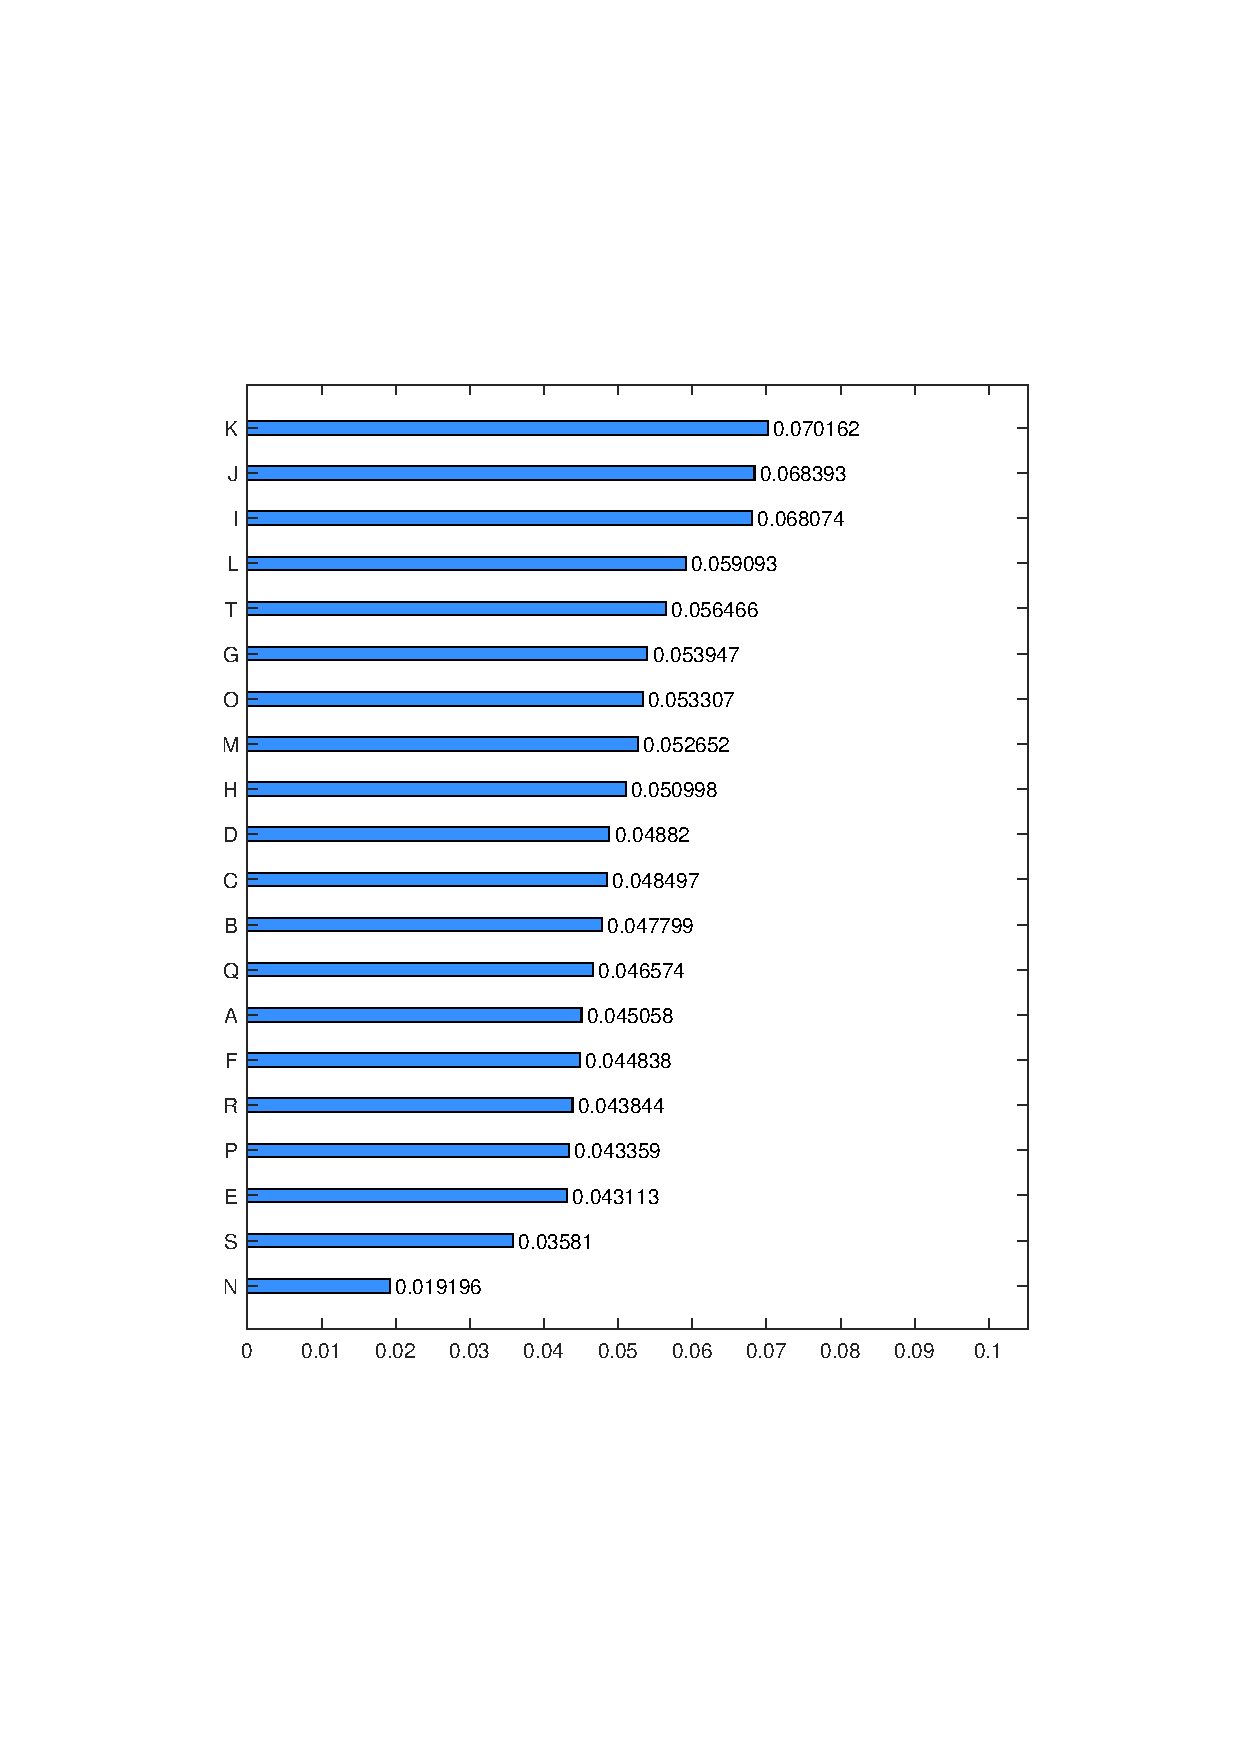
\includegraphics[width=\textwidth]{河流排名}
        \caption{河流最终得分}\label{Fig:1}
    \end{figure}

    \section{模型评价}

    \subsection{优点}
    \begin{enumerate}
        \item TOPSIS 对原始数据的利用很充分
        \item TOPSIS 对指标的分布和数量没有很大要求
    \end{enumerate}

    \subsection{局限}
    \begin{enumerate}
        \item 以上建模并未考虑指标的权重
    \end{enumerate}

    \section{模型改进}

    事实上,将距离定义改为
    $$D_i^+=\sqrt{\sum\limits_{j=1}^{n}\omega_j (Z_j^+-z_{ij})^2}$$
    $$D_i^-=\sqrt{\sum\limits_{j=1}^{n}\omega_j (Z_j^--z_{ij})^2}$$

    则可考虑指标附带权重的 TOPSIS 模型。其中的权重 $\sum\limits_{j=1}^{n} w_j=1$,可由层次分析法或熵权法等评价方法生成。

    \appendix

    \section{Matlab代码}
    \begin{lstlisting}[language=matlab,caption={TOPSISsmall.m}]
    function X = TOPSISsmall(X0,position)
    % 将极小型指标转化为极大型指标
    % X0:原始矩阵
    % position:极小型指标位置索引
    % X:转化后的矩阵
    
        for i=position
            small = X0(:,i);
            big = max(small) - small;
            X0(:,i) = big;
        end
        
        X=X0;
    end
    \end{lstlisting}

    \begin{lstlisting}[language=matlab,caption={TOPSISmiddle.m}]
    function X = TOPSISmiddle(X0,x0,position)
    % 将中间型指标转化为极大型指标
    % X0:原始矩阵
    % x0:中间值
    % position:中间型指标位置索引
    % X:转化后的矩阵
    
        %% 判断x0和position是不是一样大
        n1 = length(x0);
        n2 = length(position);
        if n1~=n2
            disp("输入的参数维数不对应!!!")
            X = [];
            return 
        end
        
        %% 转化
        for i = 1:n1
            medium = X0(:,position(i));
            M = max(abs(medium-x0(i)));
            big = 1 - abs(medium-x0(i))/M;
            X0(:,position(i)) = big;
        end
        X=X0;
    end
    \end{lstlisting}

    \begin{lstlisting}[language=matlab,caption={TOPSISrange.m}]
    function X = TOPSISrange(X0,S,E,position)
    % 将区间型指标转化为极大型指标
    % X0:原始矩阵
    % S:区间起点
    % E:区间终点
    % position:中间型指标位置索引
    % X:转化后的矩阵
    
        %% 判断x0和S和E是不是一样大
        n1 = length(S);
        n2 = length(position);
        n3 = length(E);
        if ~(n1==n2 && n1==n3)
            disp("输入的参数维数不对应!!!")
            X = [];
            return 
        end
        
        %% 转化
        for i = 1:n1
            range = X0(:,position(i));
            a = S(i);
            b = E(i);
            M = max(a-min(range),max(range)-b);
            big = ones(1,length(range));
            for j = 1:length(range)
                if range(j)<a
                    big(j)=1-(a-range(j))/M;
                elseif range(j)>=a && range(j)<=b
                    big(j)=1;
                else
                    big(j)=1-(range(j)-b)/M;
                end
            end
            X0(:,position(i)) = big;
        end
        X=X0;
    end
    \end{lstlisting}

    \begin{lstlisting}[language=matlab,caption={TOPSISnormlize.m}]
    function X = TOPSISnormlize(X0)
    % 将数据标准化
    
        n = size(X0,2);
        for i=1:n
            X0(:,i)=X0(:,i)/norm(X0(:,i));
        end
        X = X0;
    end        
    \end{lstlisting}

    \begin{lstlisting}[language=matlab,caption={TOPSISdistance.m}]
    function D = TOPSISdistance(X,b,w)
    % 计算矩阵每个行向量距离某一个向量的加权距离
    
        [m,n1] = size(X);
        n2 = length(b);
        n3 = length(w);
        if n3==0
            w = ones(n2,1);
            n3 = n2;
        end
        if ~(n1==n2 && n1==n3)
            disp("参数维数不对应");
        end
        
        w = w/sum(w);
        D = ones(m,1);
        for i=1:m
            D(i,1) = sqrt((X(i,:)-b).^2*w);
        end
    end
    \end{lstlisting}

    \begin{lstlisting}[language=matlab,caption={sortWeights.m}]
    function [sortedWeights,sortedLabels] = sortWeights(weights,labels)
    % 使用冒泡排序算法从小到大排序权重和标签
    % weights和labels应为行向量或列向量
        n = length(weights);
        
        %% 冒泡排序
        for i=1:n
            for j=1:n-i
                if weights(j)>=weights(j+1)
                tempNum = weights(j);
                weights(j) = weights(j+1);
                weights(j+1) = tempNum;
        
                tempLabel = labels(j);
                labels(j) = labels(j+1);
                labels(j+1) = tempLabel;
                end
            end
        end
        
        sortedWeights = weights;
        sortedLabels = labels;
    end        
    \end{lstlisting}

    \begin{lstlisting}[language=matlab,caption={drawWeights.m}]
    function  drawWeights(weights,labels)
    % 绘制权重图
    % weights:权重行向量或列向量
    % labels:数据标签
    
        n = length(weights);
        weights = weights / sum(weights);
        facecolor = "#3691ff";
        width = 0.3;
        barh(weights,FaceColor=facecolor,BarWidth=width);
        xlim([0,3/2*max(weights)]);
        yticks(1:n)
        yticklabels(labels);
        for i=1:n
            text(weights(i)+1/100*max(weights),i,num2str(weights(i)))
        end
    end  
    \end{lstlisting}
    

    \begin{lstlisting}[language=matlab,caption={TOPSIS主体}]
    clc,clear

    %% 导入数据
    waterMatrix = readmatrix("data\水质数据.csv");
    
    %% 确定指标类型
    % 极小型
    smallIndex = 3;
    % 中间型
    mediumIndex = 2;
    x0 = 7;
    % 区间型
    rangeIndex = 4;
    S = 10;
    E = 20;
    
    %% 指标正向化
    waterMatrix = TOPSISsmall(waterMatrix,smallIndex);
    waterMatrix = TOPSISmiddle(waterMatrix,x0,mediumIndex);
    waterMatrix = TOPSISrange(waterMatrix,S,E,rangeIndex);
    
    %% 标准化
    waterMatrix = TOPSISnormlize(waterMatrix);
    
    %% 计算得分并归一化
    best = max(waterMatrix);
    worst = min(waterMatrix);
    Db = TOPSISdistance(waterMatrix,best,[]);
    Dw = TOPSISdistance(waterMatrix,worst,[]);
    weights = Dw./(Db+Dw);
    weights = weights/sum(weights);
    [weights,labels] = sortWeights(weights,["A","B","C","D","E","F","G","H","I" ...
        ,"J","K","L","M","N","O","P","Q","R","S","T"]);
    drawWeights(weights,labels)
    \end{lstlisting}

    \section{Python 代码}

    \begin{lstlisting}[language=python ,caption={参数初始化} ]
    ## 导包
    import numpy as np
    import matplotlib.pyplot as plt
    import pandas as pd
    
    np.set_printoptions(suppress=True)
    
    plt.rcParams["font.sans-serif"]=["SimHei"] #设置字体
    plt.rcParams["axes.unicode_minus"]=False # 解决图像中的“-”负号的乱码问题

    ## 导入数据
    waterMatrix = pd.read_csv("../data/水质数据.csv",header=None)
    waterMatrix = waterMatrix.to_numpy()

    ## 指标类型确定
    # 极小型指标
    small = [2]
    # 中间型指标
    medium = [1]
    x0 = [7]
    # 区间型指标
    Range = [3]
    S = [10]
    E = [20]
    \end{lstlisting}

    \begin{lstlisting}[language=python ,caption={函数定义} ]
    def TOPSISsmall(X0, position):
        """将极小型指标转化为极大型指标"""
        X = X0.copy()
        for i in position:
            X[:, i] = np.max(X[:, i]) - X[:, i]
        return X


    def TOPSISmedium(X0,x0,position):
    """将中间型指标转化为极大型指标"""

        # 判断x0和position是不是一样大
        n1,n2 = len(x0),len(position)
        if n1!=n2:
            print("列表维数不对应!!!")
            return None
        
        # 转化
        X=X0.copy()
        for i in range(n1):
            medium = X[:,position[i]]
            M = np.max(np.abs(medium - x0[i]))
            X[:,position[i]]=1-np.abs(medium-x0[i])/M
        return X


    def TOPSISrange(X0, S, E, position):
    """将区间型指标转化为极大型指标"""

        # 判断n1,n2,n3是否一样大
        n1, n2, n3 = len(S), len(E), len(position)
        if not (n1 == n2 and n1 == n3):
            print("输入的参数维数不对!!!")
            return None
    
        # 转化
        X=X0.copy()
        for i in range(n1):
            Range = X[:, position[i]]
            m = np.size(Range)
            a = S[i]
            b = E[i]
            M = np.max([a-np.min(Range), np.max(Range)-b])
            big = np.ones(m)
            for j in range(m):
                if Range[j] < a:
                    big[j] = 1-(a-Range[j])/M
                elif Range[j] >= a or Range <= b:
                    big[j] = 1
                else:
                    big[j]=1-(Range[j]-b)/M
            X[:,position[i]] = big
        
        return X

    def TOPSISnormlize(X0):
    """矩阵标准化"""
        
        X = X0.copy()
        n = X.shape[1]
        
        for i in range(n):
            X[:,i] = X[:,i] / np.linalg.norm(X[:,i])
        
        return X


    def TOPSISdistance(X, b, w=None):
    """计算一个矩阵的每个行向量与某个向量的加权距离"""
    
        m, n1 = X.shape
        n2 = np.size(b)
    
        if type(w) != np.array:
            w = np.ones(n2)
            n3 = n2
        n3 = np.size(w)
    
        if not (n1 == n2 and n1 == n3):
            print("输入的参数维数不对!!!")
            return None
    
        w = w / np.sum(w)
        D = np.ones(m)
        for i in range(m):
            D[i] = np.sqrt(np.dot(np.dot(X[i, :]-b, X[i, :]-b), w))[0]
            
        return D
    
    
    def sortWeights(weights, labels):
    """从小到大排序权重和标签"""

        weights = weights / sum(weights)
        wl = list(zip(weights, labels))
        wl.sort(key=lambda x: x[0])
        sortedWeights, sortedLabels = zip(*wl)
        sortedWeights = np.array(sortedWeights)
        sortedLabels = list(sortedLabels)
        return sortedWeights, sortedLabels


    def drawWeights(weights, labels, height=0.2):
    """绘制权重图"""
        n = len(weights)
        ax = plt.axes()
        ax.set_facecolor("#FAFAF8")
        ax.barh([i for i in range(1,
                                  len(weights) + 1)],
                weights,
                height=height,
                color="#3691ff")
        y = [i for i in range(1, n + 1)]
        plt.yticks(y, labels)
        plt.xlim(0, 4/3*np.max(weights))
        for i in range(n):
            plt.text(weights[i] + 1/100*np.max(weights),
                     y[i], np.around(weights[i], 4), ha="left", va="center")
    \end{lstlisting}

    \begin{lstlisting}[language=python ,caption={TOPSIS主体} ]
    # 指标正向化
    waterMatrix = TOPSISsmall(waterMatrix, small)
    waterMatrix = TOPSISmedium(waterMatrix, x0, medium)
    waterMatrix = TOPSISrange(waterMatrix, S, E, Range)
    
    # 标准化
    waterMatrix = TOPSISnormlize(waterMatrix)
    
    # 计算得分并归一化
    best = np.max(waterMatrix,0)
    worst = np.min(waterMatrix,0)
    Db = TOPSISdistance(waterMatrix, best)
    Dw = TOPSISdistance(waterMatrix, worst)
    weights = Dw / (Db + Dw)
    weights = weights / np.sum(weights)
    [weights, labels] = sortWeights(weights, ["A", "B", "C", "D", "E", "F",
                                    "G", "H", "I", "J", "K", "L", "M", "N", "O", "P", "Q", "R", "S", "T"])
    drawWeights(weights,labels,0.7)
    \end{lstlisting}
\end{document}